\documentclass[a4paper,12pt]{article}
\usepackage[left=0.75in,right=0.75in,top=1.5in,bottom=1.5in,footskip=.25in]{geometry}
\usepackage{graphicx}
\usepackage[english]{babel}
\usepackage[utf8x]{inputenc}
\usepackage{url}
\usepackage[ruled]{algorithm2e}
\usepackage{array}

\newcommand{\Name}{Jhanvi Arora}
\newcommand{\ProjectName}{Calculate: CosInverse (Arccos(x))}
\newcommand{\ProblemName}{Problem 1}
\newcommand{\Title}{}
\newcommand{\Course}{\textbf{SOEN-6011 \vspace{0.5cm} Software Engineering Processes}}
\newcommand{\ProfessorName}{Dr. Pankaj Kamthan}

\begin{document}

%----------------------------------------------------------------------------------------
% TITLE PAGE START
%----------------------------------------------------------------------------------------

\begin{titlepage}
\newcommand{\HRule}{\rule{\linewidth}{0.2mm}} %New command for thickness of line


\centering

\includegraphics[scale=.35]{concordia.png}\\[1cm]
\textsc{\Large \Course} \\ [0.5cm]

%--------
% TITLE
%--------

{ {\huge{\textbf{\ProjectName}}} 


%---------
% TAIL SECTION
%---------

\vspace{8cm}
\Large \textsc{\textbf{Professor: \ProfessorName}}\\
\Large \textsc{\textbf{Submitted by: \Name}}\\
\vfill
}
\end{titlepage}





\pagebreak
%----------------------------------------------------------------------------------------
% Report START
%----------------------------------------------------------------------------------------


%---------
%SECTION 1
%---------
\section{Problem: Arccosine(x)}
    \subsection{Description \cite{Arc cosine}}
    Compute the value of arccos(x) for any given number x with minimum absolute error difference in resemblance to scientific calculators, given x satisfies the domain requirements of the aforementioned function.
    \begin{figure}[htp]
     \centering
     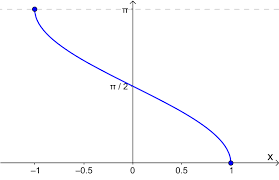
\includegraphics[scale=1]{download.png}\\[1cm]
     \label{fig:graph}
     \caption{Graph of function ($\arccos(x), x$)}
    \end{figure}

From the above graph \ref{fig:graph} following properties of function are inferred:
    \begin{itemize}
        \item {It is decreasing function.}
        \item{It has no mirror image across x axis nor in y-axis.}
    \end{itemize}
    \subsection{Domain}
    {For function, \[y = arccos(x)\]:
    \newline
    The value of x should satisfy: 
    \begin{math}
    {\quad x  \in  R, \quad -1 \leq x \leq 1}
    \end{math}
    }
    \subsection{Co-domain}
    {For function, \[y = arccos(x)\]
    \newline
    The value of y should satisfy:
    \begin{math}
    {\quad y \in R, \quad 0 \leq y \leq \pi}
    \end{math}
    }

\pagebreak

\section{Context-Use-Model}
In the following environment scenarios, the various interactions with the developed system are described as follows:
    \subsection{Technical Environment}
    \begin{enumerate}
    \item{Developers: \\[1\baselineskip] Understand reusability and maintainability of modules in the calculators }
    \item{Testers: \\[1\baselineskip] Understand and test functionality of modules.}
    \item{DevOps Personnel: \\[1\baselineskip] Setup and maintain the CI/CD pipeline for the developed system and handle its deployment options. }
    \end{enumerate}
    \subsection{Non-Technical Environment}
    \begin{enumerate}
        \item {Students: \\[1\baselineskip] University and high school students whose coursework include math/math-based functions}
        \item{Architects and Design Planners: \\[1\baselineskip] Planning of various construction sites, determine elevation and tilt requires use of the function.}
        \item{Mathematicians: \\[1\baselineskip]  Apply the output results to derive their implications. }
    \end{enumerate}

\section{Functional Requirements}
    \subsection{Assumptions}
    \begin{itemize}
        \item {ID: A1 \\[1\baselineskip] Input is a real number.}
        \item {ID: A2 \\[1\baselineskip] The results are precise upto 6 decimal places.}
        \item{ID: A3 \\[1\baselineskip] The scientific calculator derived input constants used in function calculations are correct.}
    \end{itemize}
    \subsection{Requirements}
    \begin{itemize}
        \item {ID: R1 
        \begin{itemize}
            \item {Version: 1.0}
            \item{Type: Functional Requirement}
            \item{Priority: 1}
            \item {Risk: High.}
            \item{Description: Should not accept any out of defined-domain values.}
            \item{Rationale: Function undefined for out-of-domain values.}
        \end{itemize}}
        \item {ID: R2 
        \begin{itemize}
            \item {Version: 1.0}
            \item{Type: Functional Requirement}
            \item{Priority: 1}
            \item {Risk: High.}
            \item{Description: Result should not be out of bounds of co-domain.}
            \item{Rationale: Output of function is fixed within its co-domain.}
        \end{itemize}}
        \item {ID: R3 
        \begin{itemize}
            \item {Version: 1.0}
            \item{Type: Functional Requirement}
            \item{Priority: 2}
            \item {Risk: Low.}
            \item{Description: Error should be in  [0, 0.0001] }
            \item{Rationale: It should provide precision upto atleast 4 decimal places.}
        \end{itemize}}
        \item {ID: R4 
        \begin{itemize}
            \item {Version: 1.0}
            \item{Type: Functional Requirement}
            \item{Priority: 3}
            \item {Risk: Low.}
            \item{Description: Display result in degree.}
            \item{Rationale: Some applications require degree output instead of default radians.}
        \end{itemize}}
        \item {ID: R5 
        \begin{itemize}
            \item {Version: 1.0}
            \item{Type: Non Functional Requirement}
            \item{Priority: 3}
            \item {Risk: Low.}
            \item{Description: Yield output in lowest time.}
            \item{Rationale: To function as Calculator it should provide output in milliseconds.}
        \end{itemize}}
    \end{itemize}
\pagebreak

\section{Algorithm}
    \subsection{Main Algorithm}
    \begin{algorithm}
    \caption{Fast Arc Cosine Algorithm \cite{Abramowitz Book}.}
    \KwData{$-1 \leq x \leq 1$}
    \KwResult{$y = arccos(x)$}
    \eIf{$x<0$}{$negative \gets 1$}{$negative \gets 0$}
    \If{$(x==1)$}{$y=0$}
    \If{$(x==-1)$}{$y= \pi$}
    \If{$(x<-1) | (x>1) $}{$y= -1$}
    \If{$(x<-0) $}{$x=x*-1$}
    $result \gets  fv1$\;
    $result \gets result*x$\;
    $result \gets result +  fv2$\;
    $result \gets result*x$\;
    $result \gets result + fv3$\;
    $result= result*x$\;
    $result \gets result + fv4$\;
    $result \gets result* squareRoot(1-x)$\;
    $result \gets result- 2*negative*result$\;
    $y \gets negative * \pi + result$\;
    \end{algorithm}
    \pagebreak
    
    
    \begin{algorithm}
    \caption{SquareRoot}
    \KwData{$x>0$}
    \KwResult{$y = squareRoot(x)$}
    $y = x/2$\;
    $temp \gets None$\;
    \While{$temp-y==0$}{
        $temp \gets y$\;
        $y=(temp+(x/temp))/2$;
    }
    \end{algorithm}
    
    \begin{algorithm}
    \caption{Radian To Degree}
    \KwData{$x in rad$}
    \KwResult{$y = degree(x)$}
    $y = x * 180/\pi$\;
    \end{algorithm}
\subsection{Description}
    The aforementioned algorithm is an implementation of the arc cosine derived by the approximation expansion of taylor series of arccos(x) -\cite{Abramowitz Book}. It has several constant approximation values that are used in calculations at each step- the sub functions used in approximation process are squareRoot and absolute which are a part of the developed system in code.
\subsection{Algorithm Choices}
    The options to choose from while implementing the function :
    \begin{itemize}
    \item{\textbf{Fast Arc Cosine Algorithm\cite{Abramowitz Book}.} \newline \underline{Advantages}}
    \begin{itemize} 
        \item {Approximation Algorithm - hence with derived memory constants takes lesser time.}
        \item{Uses less number of memory constants in comparison to Strict Math Algorithm .}
    \end{itemize}
    \underline{Disadvantages}
    \begin{itemize}
        \item {Precision upto only 5 decimal values. However in terms of requirements, it satisfies R3 and even satisfies R5 better than Strict Math.}
    \end{itemize}
    \item{\textbf{Strict Math Approximation Algorithm \cite{Strict Math}.}}
    \newline
    \underline{Advantages}
    \begin{itemize}
        \item {Use of memory constants and no dependency on other functions.}
        \item{Provides precision upto 8 decimal places.}
    \end{itemize}
    \underline{Disadvantages}
    \begin{itemize}
        \item {Takes more time than Strict Fast Arc Cosine.}
        \item{Requires a lot of memory for saving up precise constants.}
    \end{itemize}
    \item{\textbf{Value of arccos(x) derived from arctan(x) \cite{Taylor Series Expansion}.}}
    \newline
    \underline{Advantages}
    \begin{itemize}
        \item {arctan(x) is easier to obtain in terms of taylor series expansion.}
    \end{itemize}
    \underline{Disdvantages}
    \begin{itemize}
        \item {Time taking Recursive Function.}
        \item{Not exact Approximation in comparison to other two algorithms.}
    \end{itemize}
    \end{itemize}
    
    The first two algorithms are both approximation based approaches with fixed constant values and defined set of calculations. The third approach is polynomial based approach which entails the calculation of arctan(x) first and then using the approximated value it derives the value of arccos(x).
    
    Strict Math was initially implemented while developing the calculation system. However owing to time of yielding result and space to save up constants - Fast Arc Cosine was instead preferred.

\section{Implementation}
The implementation of the described function using the aforementioned Algorithm is carried out using Java. The project work for the same is carried out on JetBrains IntelliJ, however it is developed independent of the IDE environment. Hence, can be run on any compatible systems.

The functions used in the code do not make use of any Java in-built libraries, the math functions used in the function are implemented using code. 
\subsection{Debugger}
The debugger used in the system development is IntelliJ IDE's inbuilt debugger - which automates the process of debugging by providing multiple options of evaluating various breakpoints.
    \begin{figure}
     \centering
     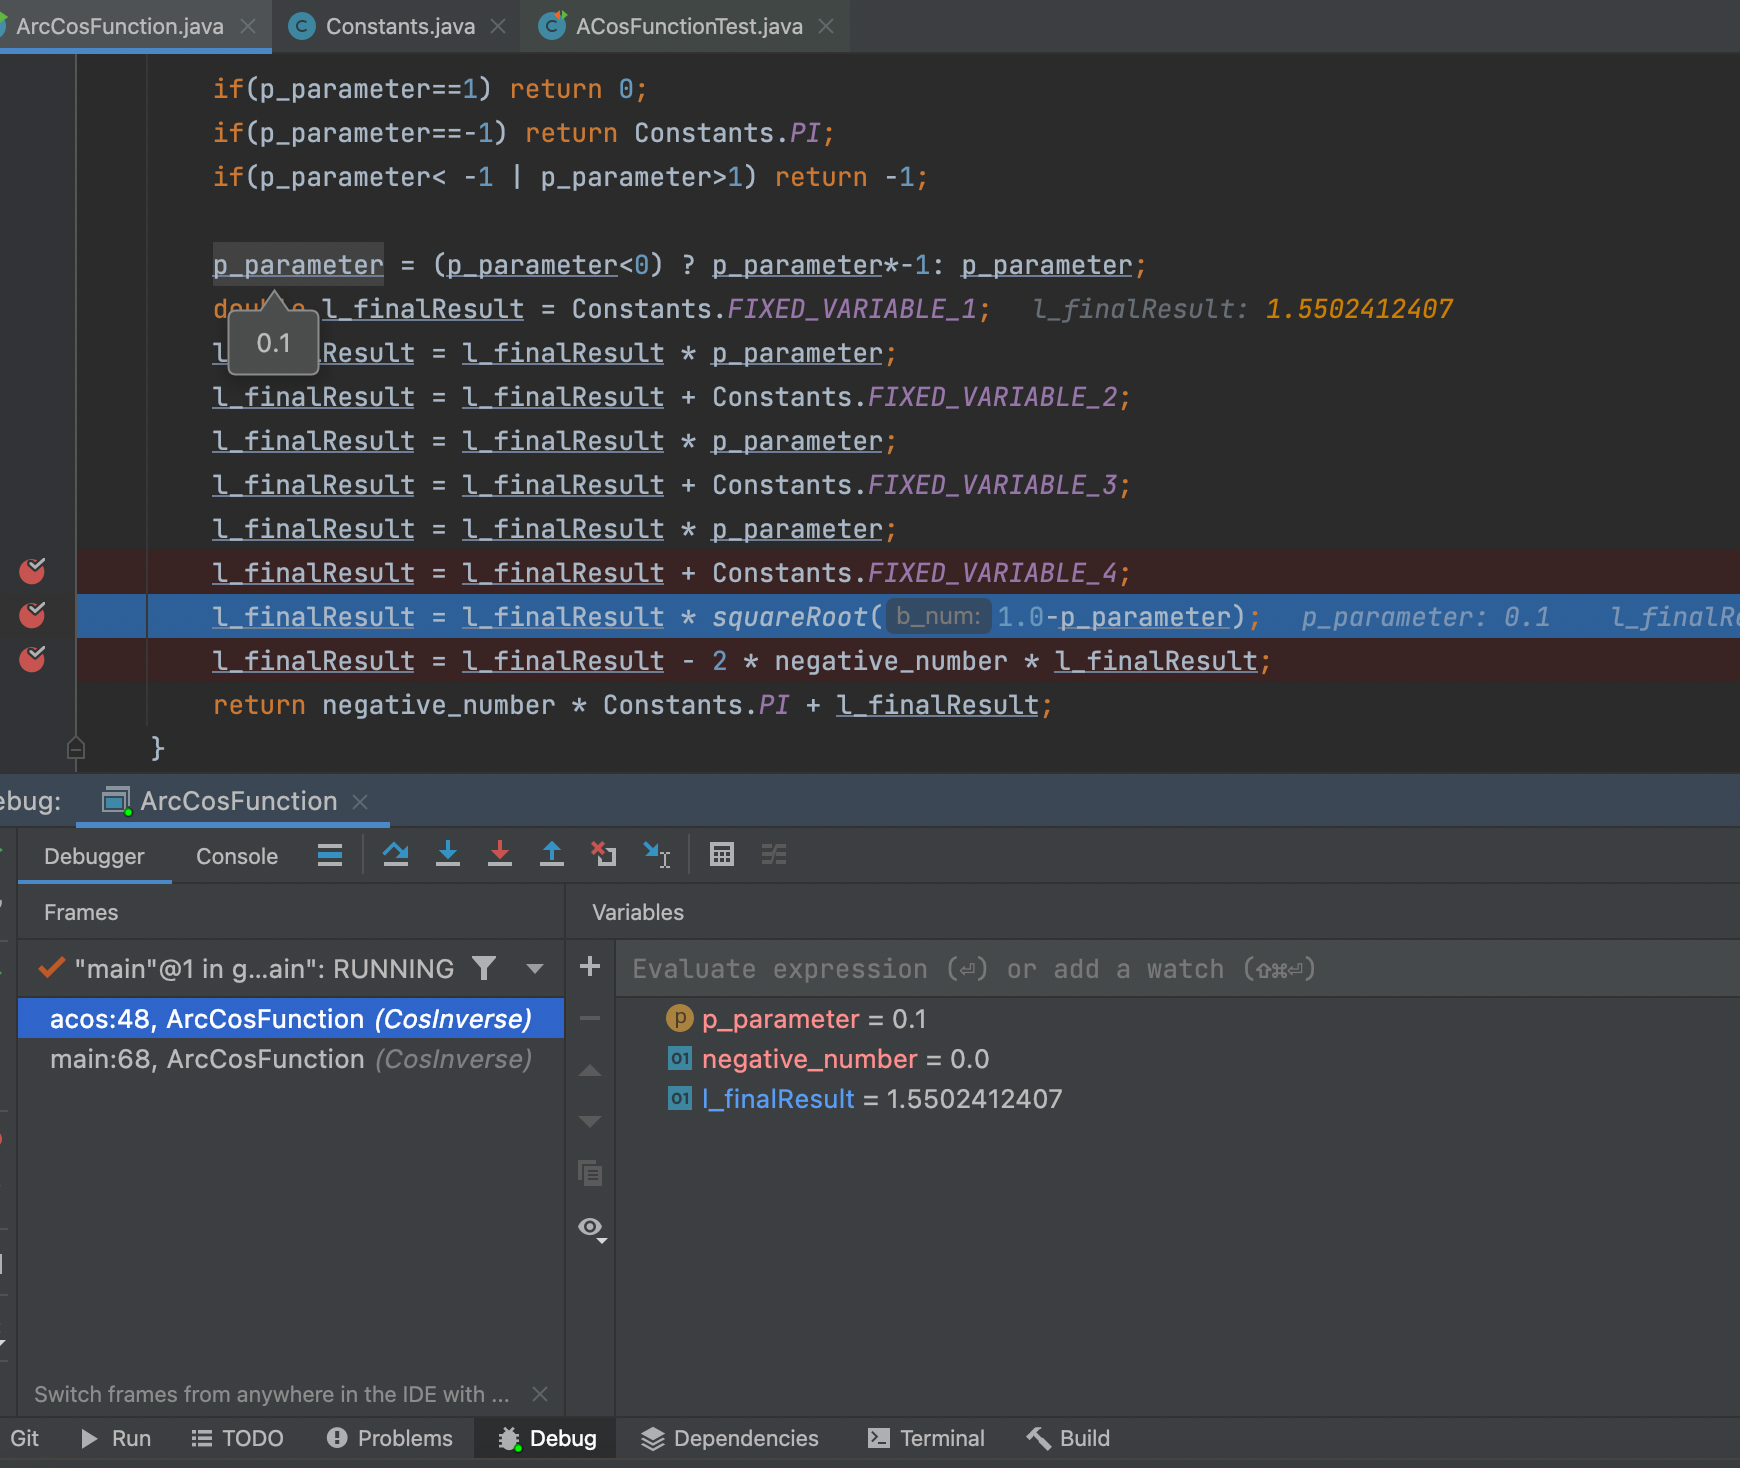
\includegraphics[scale=0.45]{Line.png}
     \caption{Evaluation of Line Breakpoint}
     \centering
     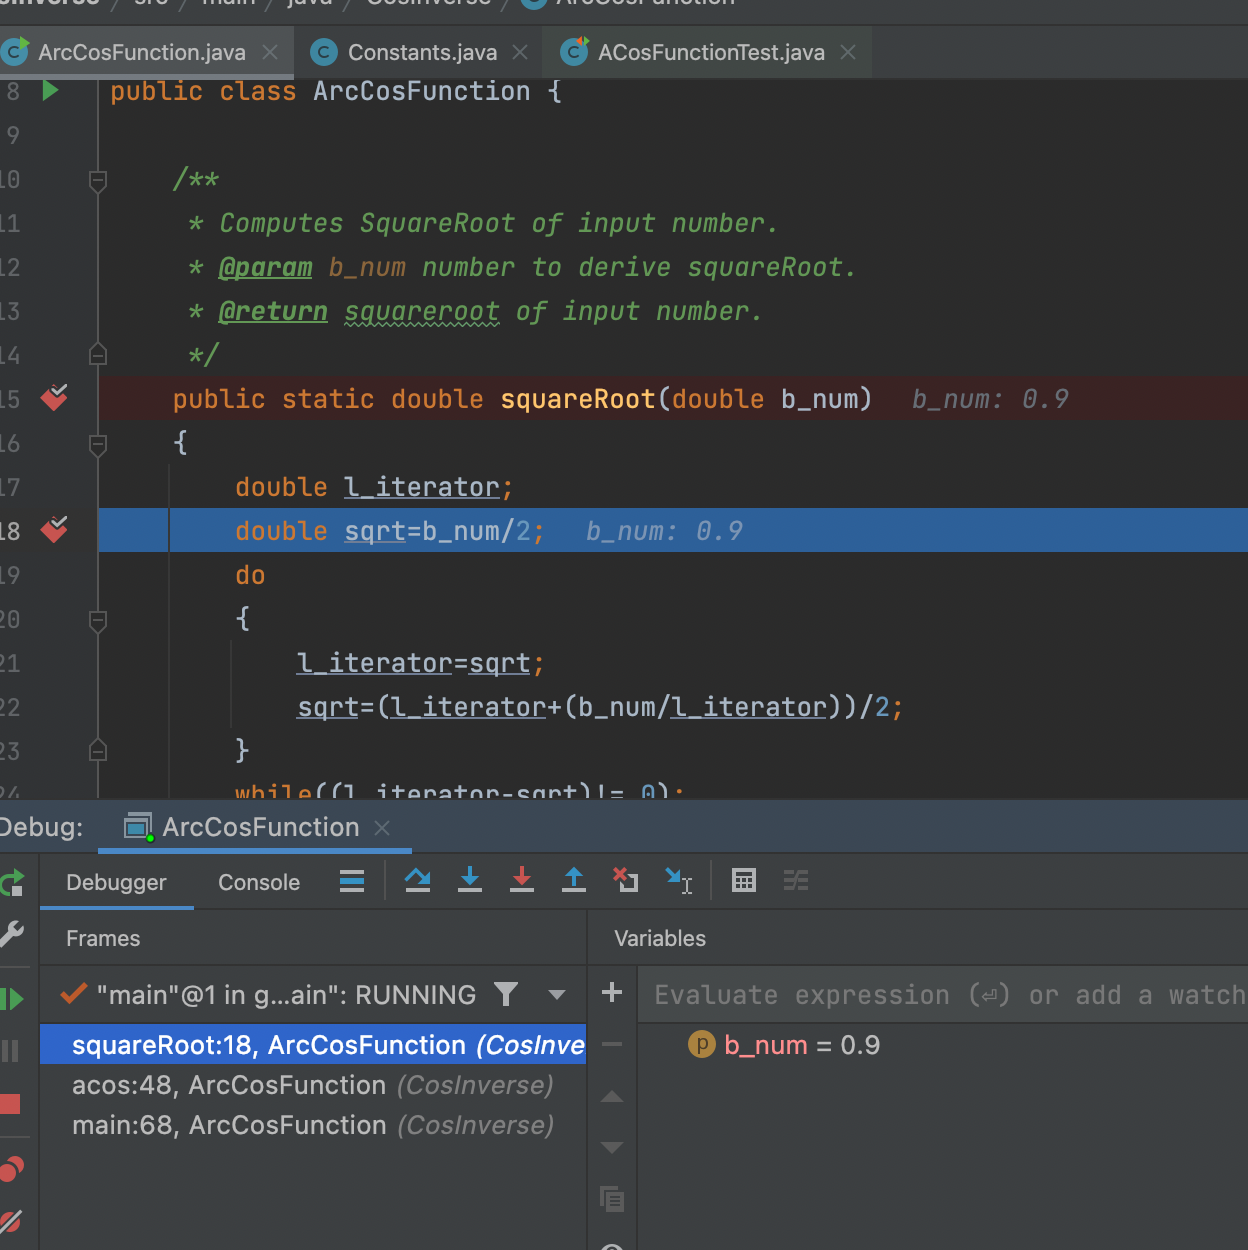
\includegraphics[scale=0.5]{Method.png}
     \caption{Evaluation of Method Breakpoint}
    \end{figure}

    \underline{Advantages}
    \begin{itemize}
        \item {Selects breakpoints on its own when called upon a function.}
        \item{Can Step out of the breakpoint - when necessary.}
        \item{Update the value of the data attributes while in debug mode.}
    \end{itemize}
    \underline{Disadvantages}
    \begin{itemize}
        \item {Difficult to analyze big volumes of code.}
        \item{Doesn't trace data-flow when it comes from different modules.}
    \end{itemize}
As in Figure- the debugging of line breakpoints causes the debugger to display the current state information of all variables at that time. The method breakpoint implies all the functional lines of the code are set as breakpoints by default and we can monitor at each the step the contents of various data parameters.
\subsection{Code Quality}
The following enumerates the code quality characteristics ensured while implementation of the calculator function:
    \begin{enumerate}
        \item \textbf{Space Efficient}\newline
        \underline{Effort:} Used the algorithm that uses lesser number of memory constants.
        \item\textbf{Portable}\newline
        \underline{Effort:} Complete implementation of the function is encased in a class that is just dependent on the Constants - hence can be plugged in to create a object and calculate values as and when needed.
        \item\textbf{Maintainable}\newline
        \underline{Effort:} The functions of the code are reusable and are independent of each other and hence any changes in the one won't affect the other.
        \item\textbf{Correctness}\newline
        \underline{Effort:} Each of the functions are tested for all possible input cases to verify the working.
        \item\textbf{Robustness}\newline
        \underline{Effort:} The code is robust and handles all the input yielding correct outputs in reference to the given requirements.
        \item\textbf{Time-Efficient}\newline
        \underline{Effort:} Over the use of recursive and calculation extensive method algorithms as in previous section- the most efficient and less time taking algorithm is implemented.
         \item\textbf{Usable}\newline
        \underline{Effort:} The functions can be immediately accessed by calling upon the object of the class - hence the implemeneted system is fully usable.
    \end{enumerate}
\pagebreak
\subsection{Checkstyle \cite{Checkstyle}}
Checkstyle is a tool that imposes programming code style check on the source code. 
    \begin{itemize}
        \item {It is to ensure that the written code conforms to the quality measures as defined by the standards.}
        \item{The programming style conventions checked for by the checkstyle are Google Java Programming Standards.}
        \item{The aforementioned is imposed using the Maven framework using which the project is initialised. }
    \end{itemize}
    \textbf{Advantages}
    \begin{itemize}
     \item{It prompts on any inefficient coding- convention followed.}
     \item{It is automated and checks the whole project build on one command.}
     \item{Custom - Quality Conventions can also be instilled in Checkstyle to ensure them.}
    \end{itemize}
    \textbf{Disadvantages}
    \begin{itemize}
     \item{It doesn't prompts immediately - but when run on the whole project}
     \item{It requires the code to be compiled by the compiler.}
     \item{Refactored or ill-structured code aren't checked by checkstyle.}
    \end{itemize}
    \begin{figure}
     \centering
     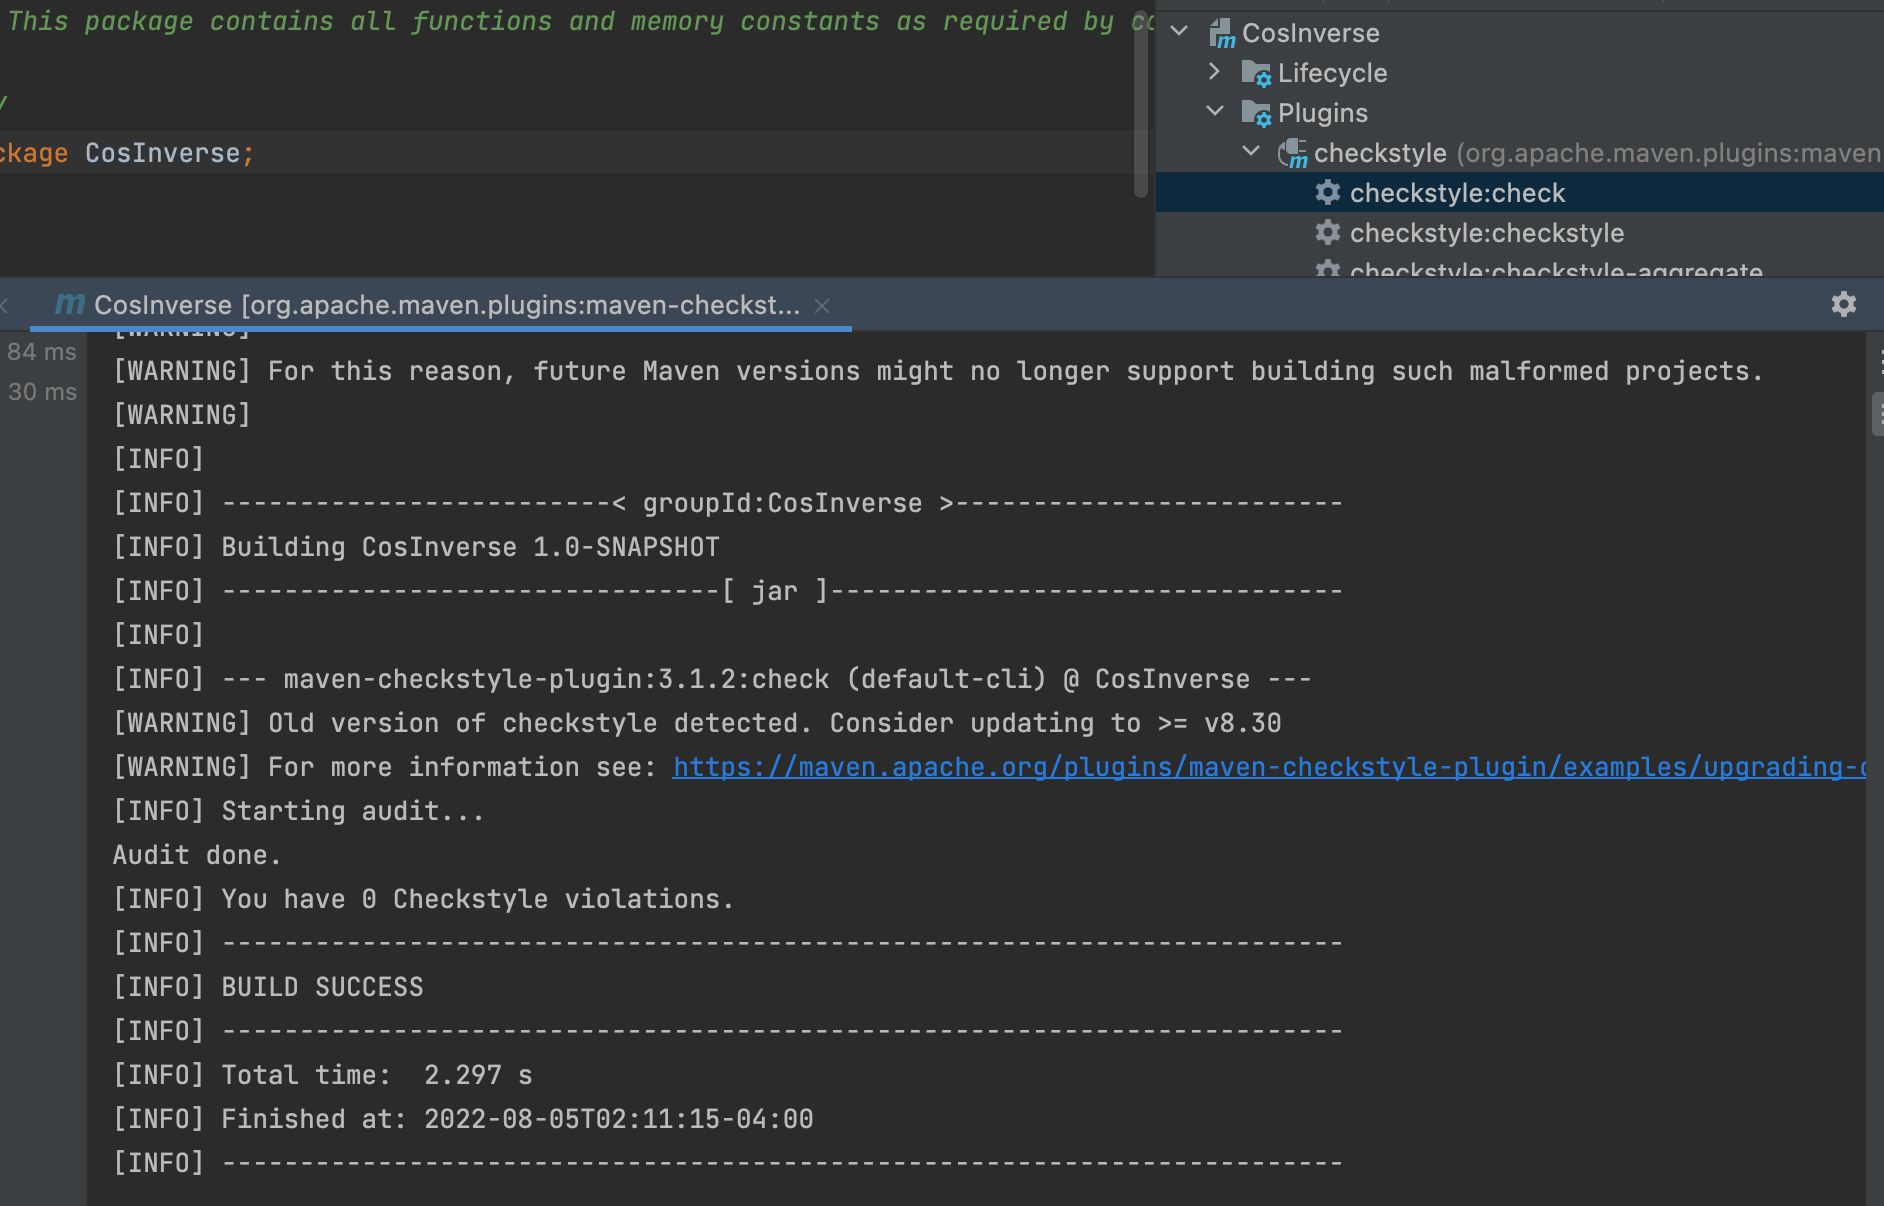
\includegraphics[scale=0.5]{Check.png}
     \caption{Snapshot of Checkstyle after completion}
    \end{figure}
    
\pagebreak

\section{Testing}
    \begin{itemize}
        \item {The testing of the implemented system has been performed using the JUnit framework 4.13.2 and was installed using the maven dependency.}
        \item{The test cases for all functions and each of their possible scenarios is included, verified and checked.}
    \end{itemize}

    \begin{table}[h]
    \centering
    \begin{tabular}{|c |c| c|} 
    \hline
     Requirement & Test Name & Description \\ [0.5ex] 
    \hline
    R1 & testOutOfRange, testWrongInput & O/p not defined for out of bound values.\\
    R2 & testpos1, testneg1 & Checks value of function at boundaries\\
    R3 & testpositive & Checks if the error delta is within 0.00001\\
    R4 & testDegreeResult & Checks if result in degree is correct\\
    \hline
    \end{tabular}
    \caption{Test Mapping to Requirements}
    \end{table}
    The implemented system passes all the aforementioned test cases henceforth satisfying all the functional requirements of the system.

\begin{thebibliography}{9}

    \bibitem{Arc cosine}
    Arc cosine, 
    \\\texttt{https://www.cuemath.com/trigonometry/arccosine/}
    
    \bibitem{Taylor Series Expansion} 
    Taylor Series Expansion,
    \\\texttt{http://scipp.ucsc.edu/~haber/ph116A/taylor11.pdf}
    
    \bibitem{Abramowitz Book}
    Abramowitz and Stegun,
    \\\texttt{https://personal.math.ubc.ca}
    
    \bibitem{Strict Math}
    Strict Math Algorithm,
    \\\texttt{https://developer.classpath.org/doc/java/lang/StrictMath-source.html}
    
    \bibitem{Checkstyle}
    Checkstyle,
    \\\texttt{https://checkstyle.sourceforge.io/}

\end{thebibliography}


\end{document}